\section{First-hierarchy 5UD-CFG embedding model}
In this section, we propose the detailed approaches how the model generates 5UD-CFG from Android apps. The traditional CFG is the common feature used in bug search. Moreover, different from other attributes on basic blocks, such as I/O pairs and statics features \cite{EschweilerYG16} \cite{PewnyGGRH17}, are more accuracy matching. Following the idea of the traditional CFG extraction, this paper utilizes CFG with different basic block level attributes with five eigenvalues called 5UD-CFG. We also prove the monotonicity of 5UD-CFG, a 5UD-CFG vector represents a CFG.


%\subsection{Disassembly of Android Application and original CFG extraction}
%In our system, the pretreatment of an application consists of disassembling the application and extracting opcode sequences. A code file is a dex file that can be transformed into smali files, where each smali file represents a single class and contains methods of such a class. Each method contains instructions and each instruction consists of a single opcode and multiple operands.  
%
%After preparation, including downloading all apps from multiple markets and extracting methods from the apps, we encode a projection form of CFG to get the unique feature of the function of an app.
%
%CFG is the control flow graph of a method. Each vertex in a CFG corresponds to a basic block in the method. A basic block is a straight-line piece of code with one entry point and one exit point. Jump targets start a block, and jump end a block. Directed edges are used to represent jumps in the control flow.
%
%Before discussing the CFG embedding, we extract the feature of basic block for each vertex in a CFG. 

Fig. 1(b) shows a primitive extracting CFG from a function. A vertex represents a basic block, and a edge represents a call link between two basic blocks. A basic block is a set of opcodes. The outgoing edges of a vertex $A$ represents the basic block $A$ is called by other basic blocks. The input edges of a vertex $A$ represent the the basic block $A$ calls other basic blocks. 

%\begin{figure}[hbt]
%  \center{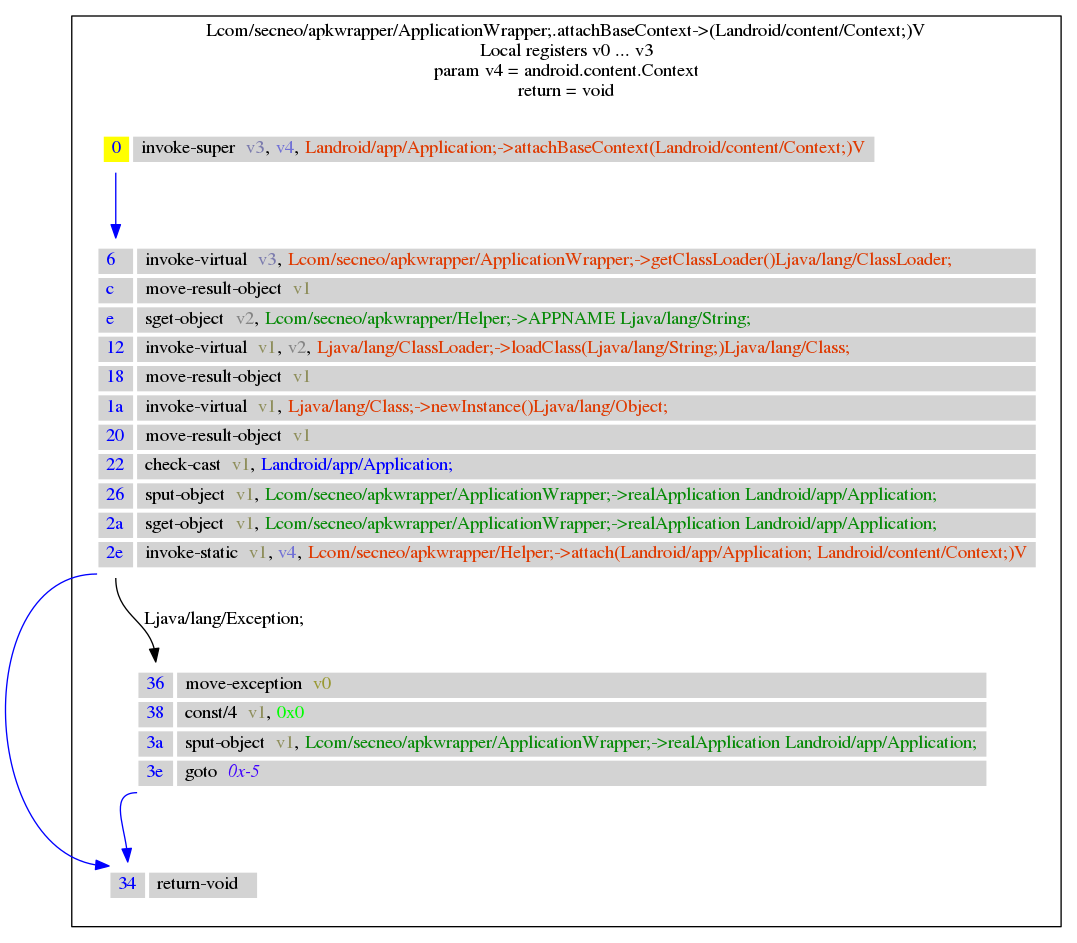
\includegraphics[width=8cm] {cfgexample.png}}
%  \caption{An example of a method CFG in a real apk}
%\end{figure}

%\subsection{Notation} 
%Before introducing the CFG embedding model, we define some of the terms and notations in Table 1 which will be used later. 
%\begin{table}[!htb]
%\newcommand{\tabincell}[2]{\begin{tabular}{@{}#1@{}}#2\end{tabular}}
%\caption{Propagation model}
%\centering
%\begin{tabular}{|l|l|}
%\hline
% Symbol& Definition \\
% \hline
% n & number of vertexes \hline
% V & vertex set of CFG\hline
%& $0.2,~ 0.5,~ 1$\\
%\hline
%The {\color{black}recovery} probability & $\mu$ & $0, ~0.5, ~1$\\
%\hline
%\tabincell{l}{The influence factor\\ of the search engine} & $\xi$ & $0.2, ~0.5,~ 1$\\
%\hline
%\tabincell{l}{The growth velocity\\ of susceptible vertexes} & r & 0.5\\
%\hline
%\tabincell{l}{The disappearing velocity\\ of susceptible vertexes} & d & 0.1\\
%\hline
%\tabincell{l}{The vanishing velocity \\ of the influence \\by the search engine} & c & 0.1\\
%\hline
%\end{tabular}
%\end{table}}

%\subsection{5UD-CFG embedding}

The main idea of 5UD-CFG embedding is to encode a CFG as a 5-dimensional vector. We use a generic nonlinear mapping to update the embedding result based on the CFG topology. 
%A new round of embedding process will start after the embedding update for all vertexes in the pervious round. 
%\end{Definition}

A 5UD-CFG can be viewed as a set of vertexes connected by edges based on the CFG topology. We need to train the vertex weight of each vertex (basic block). The vertex weight of each vertex is used to combine all vertex for representing the CFG. The embedding vector monotonously represent the CFG. We define the feature of a 5UD-CFG based on the 3D-CFG \cite{ChenLZ14}.

\textbf{Definition 6.} The feature of 5UD-CFG is a vector $<f_n, f_s, f_i, f_o, f_l>.$
\begin{equation*}
	\begin{split}
	& f_n=\frac{\sum_{e(j,k)\in CFG}(\omega_jn_j+\omega_kn_k)}{\omega},\\
	& f_s=\frac{\sum_{e(j,k)\in CFG}(\omega_js_j+\omega_ks_k)}{\omega},\\
	& f_i=\frac{\sum_{e(j,k)\in CFG}(\omega_ji_j+\omega_ki_k)}{\omega},\\
	& f_o=\frac{\sum_{e(j,k)\in CFG}(\omega_jo_j+\omega_ko_k)}{\omega},\\
	& f_l=\frac{\sum_{e(j,k)\in CFG}(\omega_jl_j+\omega_kl_k)}{\omega},\\
	& \omega=\sum_{e(j,k)\in 5UD-CFG}(\omega_j+\omega_k).\\	
	\end{split}
\end{equation*}
 where $e(j, k)$ is an edge in CFG. This edge connects two vertexes $j$ and $k$. 

The key factor of feature vector of the 5UD-CFG embedding is the vertex weight $\omega$, and we need to show the monotonicity of 5UD-CFG. For each directed edge $(i,~j)$ in CFG, we define the joint probability of the first-order call structure between vertex $v_i$ and vertex $v_j$ as follows:
\begin{equation}
  Link_1(v_i,~v_j)=\frac{1}{1+exp(\vec{x_i}^T \vec{x_j})},
\end{equation}
where $\vec{x_i} \in R_d$ is feature vector of vertex $v_i$, $\vec{x_i}=~<num_i,~squ_i, ~in_i, ~out_i, ~loop_i>$. In Eq.(1), we use the sigmod function as the embedding activation function. Eq.(1) defines a joint probability distribution of the vertex call over a CFG, and its empirical probability of two vertexes can be defined as $\widehat{Link_1}=\frac{\omega_j}{\omega_i\times W}$, where $W=\sum_{i\in V} \omega_i$ is related with the number of vertexes that call the vertex $v_i$ by the first-order call structure. To preserve the first-order call structure, we use the distance between two probability distributions to be the objective function. A straightforward way is to minimize the following objective function:
\begin{equation}
	 y_i^{(1)}=d~(\widehat{Link_1}, ~Link_1),
\end{equation}
where $d(.,.)$ is the distance between two distributions. We minimize the KL-divergence \cite{TangQWZYM15} of two probability distributions. Therefore, the objective function is:
\begin{equation}
	y_i^{(1)}=-\sum_{(i,j)\in E} s_{i,j}~ log~ Link_1~(\omega_i  v_i, ~\omega_j v_j).
\end{equation}

The second-order call structure assumes that the basic block (vertex) are invoked by the another vertexes exclude neighbors. Each basic block is also treated as a specific "contexts" of other vertexes. We define the joint probability of the second-order call structure between vertex $v_i$ and vertex $v_j$ as follows:
\begin{equation}
  Link_2(v_j|v_i)=\frac{exp(\vec{x_j}^T \vec{x_i})}{\sum_{k=1}^{|V|} exp(\vec{x_k}^T \vec{x_i})},
\end{equation}
where $|V|$ is the number of other vertexes exclude neighbor vertexes. To preserve the second-order call structure, we need to make the 
conditional distribution of  ``contexts" closed to the empirical distribution $\widehat{Link_2}~(v_j|v_i)=\frac{\omega_j}{\omega_i \times d_i}$,  where $d_i$ is the degree of vertex $i$. Therefore, we minimize the following objective function:
\begin{equation}
	 y_i^{(2)}=\sum_{i\in V}~d_i d(\widehat{Link_2},~ Link_2),
\end{equation}
where $d(.,.)$ is the distance between two distributions. We minimize the KL-divergence \cite{TangQWZYM15} of two probability distributions. Therefore, the objective function is as follows:
\begin{equation}	
	y_i^{(2)}= -\sum_{(i,j)\in E} l_{i,j}~ log~ Link_2~((\omega_j v_j) | (\omega_i v_i)),
\end{equation}
where $l_{i,j}$ is the connection between vertex $v_i$ and vertex $v_j$. If $l_{i,j}=1$, there exists a edge from vertex $i$ to $j$. If $l_{i,j}=-1$ for vertex $i$, there exists an edge from vertex $j$ to $i$. Otherwise there is no directed edge between $v_i$ and $v_j$.

To generate the CFG feature vector by preserving both the first-order and second-order call structure, we train parameters $\omega_i$ for each vertex. We adopt Maximum Likelihood Estimate for optimizing Eq (3) and (6). We sample all edges $(i,j)$ in a CFG, the gradient of weight of vertex with embedding vector $\vec{x_i}$ will be calculated as:
\begin{equation*}
	\begin{split}
	& \nabla_1 =\frac{\partial y_i^{(1)}}{\partial \omega_i}=\frac{\partial (-\sum_{(i,j)\in E} s_{i,j}~log ~Link_1(\omega_i v_i, ~\omega_j v_j))}{\partial \omega_i}\\
	& \nabla_2 =\frac{\partial y_i^{(2)}}{\partial \omega_i}=\frac{\partial (-\sum_{(i,j)\in E} s_{i,j}~log~ Link_2((\omega_j v_j) | (\omega_j v_j) ))}{\partial \omega_i}.\\
	\end{split}
\end{equation*}

%说明由于d是两个分布之间的距离,然后那个p的平均值就是empricial distribution 是wi/wj,这两个是绝对不相同,只要那个训练的向量靠近这个值,说明绝对是递增的,只用这么训练就可以了后面举个例子。
 The embedding vector space of all vertexes in a CFG is spanned by the vertex weight $W$. 
 
 In our case, we only need to ensure that it is monotonicity to embed a CFG as a vector. The gradient is used to calculate the distance between two probability distributions between original $link_{\left\{1~or~2\right\}}$ and embedding $\widehat{link_{\left\{1~or~2\right\}}}$. From Eq. (2) and Eq. (4), we know that original $link_{\left\{1~or~2\right\}}$ is monotonous. When the gradient $\nabla_1+\nabla_2 \rightarrow 0$, $link_1\approx \widehat{link_1}$ and $link_2\approx \widehat{link_2}$. The $link_1$ and $link_2$ are monotonous, so the embedding $\widehat{link_1}$ and $\widehat{link_2}$ are monotonous and $W=[\omega_1,~...,~\omega_n]$ are monotonous. Therefore, for ensuring the monotonicity of the embedding vector, we combine the gradient $\nabla=\nabla_1+\nabla_2 =0$ by the Maximum Likelihood Estimate formulas. 
 let
 \begin{equation*}
	\begin{split}
	& \frac{\partial y_i^{(1)}}{\partial \omega_i} +\frac{\partial y_i^{(2)}}{\partial \omega_i}= 0, \\
	\end{split}
\end{equation*}
 we train the parameter of the vertex weight sequence $W=[\omega_1,~\omega_2,~...,~\omega_n ] mod (n-1)$, where $n$ is the number of nodes in the CFG.

%we give an example to show how to calculate the $\omega_i$. vertex $A$ with the first sequence number is called by the vertex $B$ and the vertex $C$ directly. vertex $C$ is called by the vertex $D$ directly, and vertex $D$ is called by the vertex $E$ directly. This outgoing degree of vertex $A$ is $A_{\searrow B}^{\nearrow C \longrightarrow D \longrightarrow E}$. $A$ is related with $B$, $C$, $D$ and $E$. The result of vertex $A$ will be passed to vertex $B$ and vertex $C$. This process will also influence the vertex $D$ and $E$ by influencing the vertex $C$. 

Form above analysis, we know that the vertex weight $\omega_j$ is trained by the CFG topology $\sum_{e(j,k)\in 5UD-CFG}$, which is unique when the CFG is determined. As the view of the Definition 6, $<f_n, ~f_s, ~f_i, ~f_o, ~f_l>$ is related with $\sum_{e(j,k)\in 5UD-CFG}$. The different CFG has the different vertex weight sequence $W$. Therefore, they have different embedding vector. Fig.1 (c) shows an example of CFG that contains embedding parameters and basic blocks with features. There is an example for computing 5UD-CFG, which is shown in the appendix.

%\subsection{An example of 5UD-CFG embedding}
%we give an example to show how to calculate $\omega_i$. As shown in the Fig. 1 (c), vertex $A$ with the first sequence number is called by the vertex $B$ and the vertex $C$ directly. The vertex $C$ is called by the vertex $D$ directly, and vertex $D$ is called by the vertex $E$ directly. This outgoing degree of vertex $A$ is $A_{\searrow B}^{\nearrow C \longrightarrow D \longrightarrow E}$. $A$ is related with $B$, $C$, $D$ and $E$. The result of vertex $A$ will be passed to vertex $B$ and vertex $C$, which have a first-order call structure with vertex $A$. This process will also influence the vertex $D$ and $E$ by influencing the vertex $C$, which are the second-order call structure. 
%%\begin{figure}[hbt]
%%  \center{\includegraphics[width=8cm] {cfg.eps}}
%%  \caption{\label{1}  An example of real CFG}
%%\end{figure}
%
%Based on the above first-order call structure and the second-order call structure, the particular trained process of $W$ is as follows:
%
%\begin{eqnarray*}
%	\begin{cases}
%		\frac{\partial~Link_1^{(1)}}{\partial~\omega_1} +\frac{\partial~Link_2^{(1)}}{\partial~\omega_1}=0\\
%		\frac{\partial~Link_1^{(2)}}{\partial~\omega_2} +\frac{\partial~Link_2^{(2)}}{\partial~\omega_2}=0\\
%		\frac{\partial~Link_1^{(3)}}{\partial~\omega_3} +\frac{\partial~Link_2^{(3)}}{\partial~\omega_3}=0\\
%		\frac{\partial~Link_1^{(4)}}{\partial~\omega_4} +\frac{\partial~Link_2^{(4)}}{\partial~\omega_4}=0\\
%		\frac{\partial~Link_1^{(5)}}{\partial~\omega_5} +\frac{\partial~Link_2^{(5)}}{\partial~\omega_5}=0.\\
%		%\omega=4+0+2+1+0=7.
%	\end{cases}
%\end{eqnarray*}
%
%let $log(1+exp \left\{ k\times \omega_i \times \omega_j \right\} )=k\times \omega_i \times \omega_j$ and the weight of final vertex $\omega_5=0$, we have
%\begin{eqnarray*}
%	\begin{cases}
%		9\omega_2+10\omega_4+6\omega_5=0 \\
%		35\omega_3+37\omega_4+18\omega_5-18\omega_1=0 \\
%		20\omega_5+35\omega_2-18\omega_1=0 \\
%		25\omega_5+37\omega_2+10\omega_1-60\omega_3=0 \\
%		20\omega_3+6\omega_1+18\omega_2-50\omega_4=0 \\
%		W={\omega_1, \omega_2,\omega_3,\omega_4,\omega_5 }~mod~4.
%	\end{cases}
%\end{eqnarray*}
%
%We obtain the $W=[1,~2,~3,~1,~0].$
%
% Based on the Definition 6, we calculate the feature of a 5UD-CFG as follows:
%\begin{eqnarray*}
%	\begin{cases}
%	    \omega=1+2+3+1+0=7. \\
%		f_n=\frac{1\times 2\times 1+ 2\times 1\times 2+3\times 2\times3+ 4\times 2\times 1 +5\times 1 \times 0}{1+2+3+1+0}=4.57\\
%		f_s=\frac{1\times 2\times 1+ 7\times 1\times 2+4\times 2\times3+ 4\times 2\times 1 +1\times 1 \times 0}{1+2+3+1+0}=6.857\\
%		f_i=\frac{0\times 2\times 1+ 1\times 1\times 2+1\times 2\times3+ 1\times 2\times 1 +1\times 1 \times 0}{1+2+3+1+0}=1.429\\
%		f_o=\frac{0\times 2\times 1+ 2\times 1\times 2+1\times 2\times3+ 1\times 2\times 1 +0\times 1 \times 0}{1+2+3+1+0}=1.714\\
%		f_l=\frac{0\times 2\times 1+ 0\times 1\times 0+0\times 2\times2+ 0\times 2\times 1 +0\times 1 \times 0}{1+2+3+1+0}=0.\\
%		
%	\end{cases}
%\end{eqnarray*}


%\begin{figure}[hbt]
%  \center{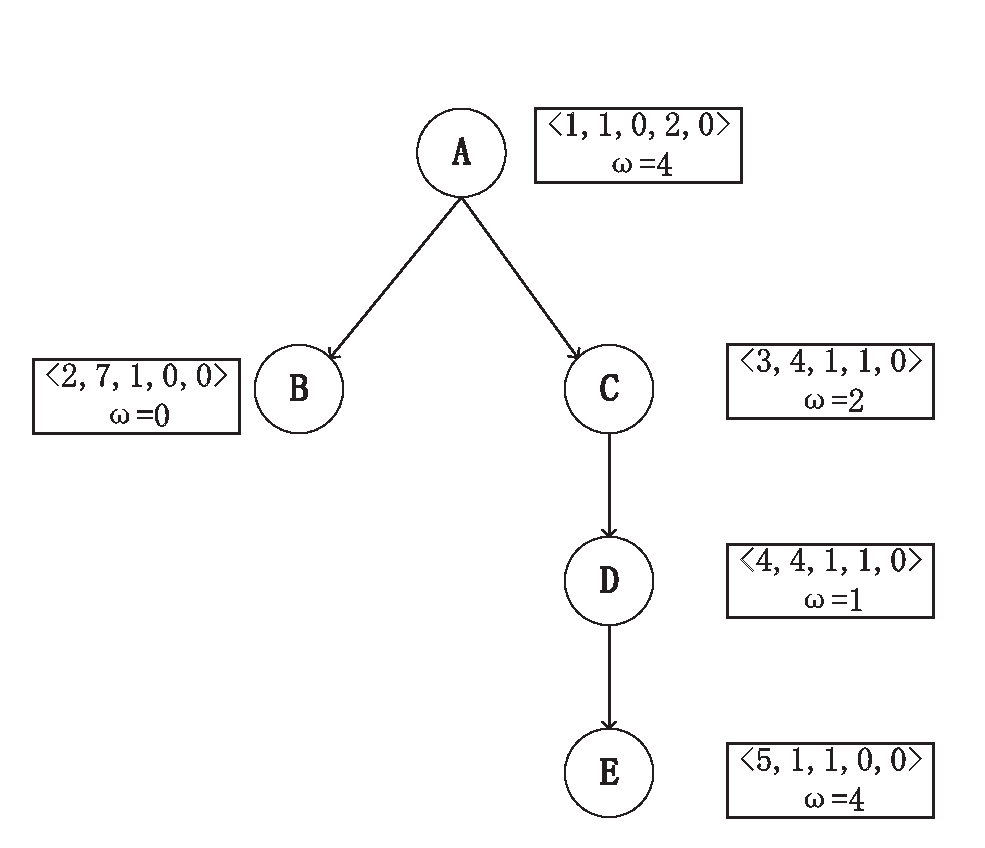
\includegraphics[width=8cm] {feature.eps}}
%  \caption{\label{1}  An example of feature of 5UD-CFG}
%\end{figure}
